\chapter{Simulation}\label{ch10}
\section{Introduction}

One of the important benefits of using a simulator like \Le is that a circuit designer can simulate digital systems to determine logic flaws or weaknesses that must be addressed before a physical \ac{IC} is manufactured. This chapter introduces the concept of simulation and includes several examples of simulated systems.

%***************************************************************************
% Section: Finite State Machines
%***************************************************************************
\section{Finite State Machines}
\label{SIM:sec:finite_state_machines}

\subsection{Introduction}
\label{SIM:subsec:intro_to_finite_state_machines}

%TODO: Maybe expand this to include Unified Modeling Language???

Sequential logic circuits are dynamic and the combined inputs and outputs of the circuit at any given stable moment is called a \emph{state}. Over time, a circuit changes states as triggering events take place. As an example, a traffic signal may be green at some point but change to red because a pedestrian presses the  ``cross'' button. The current state of the system would be ``green'' but the triggering event (the ``cross'' button) changes the state to ``red.'' 

The mathematical model of a sequential circuit is called a \ac{FSM}. A \acl{FSM} is an abstract model of a sequential circuit where each state of the circuit is indicated by circles and various triggering events are used to sequence a process from one state to the next. The behavior of many devices can be represented by a \acl{FSM} model, including traffic signals, elevators, vending machines, and robotic devices. \aclp{FSM} are an analysis tool that can help to simplify sequential circuits. 

There are two fundamental \ac{FSM} models: Moore and Mealy. These two models are generalizations of a state machine and differ only in the way that the outputs are generated. A Moore machine generates an output as a function of only the current state while a Mealy machine generates an output as a function of the current state plus the inputs into that state. Moore machines tend to be safer since they are only activated on a clock pulse and are less likely to create unwanted feedback when two different modules are interconnected; however, Mealy machines tend to be simpler and have fewer states than a Moore machine. Despite the strengths and weaknesses for each of these two \acp{FSM}, in reality, they are so similar that either can be effectively used to model any given circuit and the actual \ac{FSM} chosen by the designer is often little more than personal preference. 

\subsection{Moore Finite State Machine}
\label{SIM:subsec:moore_finite_state_machine}

The Moore \ac{FSM} is named after Edward F. Moore, who presented the concept in a $ 1956 $ paper, \emph{Gedanken-experiments on Sequential Machines}. The output of a Moore \ac{FSM} depends only on its current state. The Moore \ac{FSM} is typically simpler than a Mealy \ac{FSM} so modeling hardware systems is usually best done using a Moore \ac{FSM}. 

As an example of a Moore \ac{FSM} imagine a simple candy vending machine that accepts either five cents or ten cents at a time and vends a handful of product when $ 15 $ cents has been deposited (no change is returned). Figure \ref{SIM:fig:moore_vending_machine_fsm} is a Moore \ac{FSM} diagram for this vending machine.

\begin{figure}[H]
  \caption{Moore Vending Machine FSM}
  \label{SIM:fig:moore_vending_machine_fsm}
  \myfloatalign
  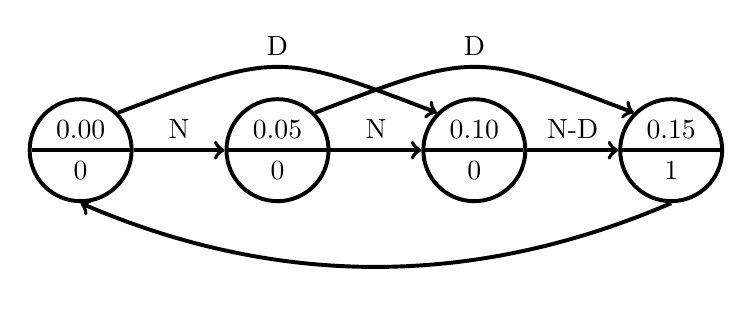
\begin{tikzpicture} [scale=1.00]
  \usepgflibrary{shapes.multipart} % for the multipart nodes
  % make all path lines (the node shapes) a little thicker
  \tikzstyle{every path}=[line width=0.50mm]  
  
  % Draw the lines
  \node [circle split,draw] (00) at (2.00, 4) {$ 0.00 $ \nodepart{lower} $ 0 $};
  \node [circle split,draw] (05) at (4.50, 4) {$ 0.05 $ \nodepart{lower} $ 0 $};
  \node [circle split,draw] (10) at (7.00, 4) {$ 0.10 $ \nodepart{lower} $ 0 $};
  \node [circle split,draw] (15) at (9.50, 4) {$ 0.15 $ \nodepart{lower} $ 1 $};
  
  % ``N'' Arrows
  \draw[->] (00.east) .. controls (3.25,4)  .. node[above] {N} (05.west);
  \draw[->] (05.east) .. controls (5.75,4)  .. node[above] {N} (10.west);
  \draw[->] (10.east) .. controls (8.25,4)  .. node[above] {N-D} (15.west);
  
  % ``D'' Arrows
  \draw[->] (00.north east) .. controls (4.50,5.25)  .. node[above] {D} (10.north west);
  \draw[->] (05.north east) .. controls (7.00,5.25)  .. node[above] {D} (15.north west);
  
  % ``Vend'' Arrow
  \draw[->] (15.south) .. controls (7.00,2.25) and (4.50,2.25)  .. node[below] {} (00.south);  
  ;
  \end{tikzpicture}
\end{figure}

In Figure \ref{SIM:fig:moore_vending_machine_fsm}, imagine that five cents is deposited between each state circle (that action is indicated by the arrows labeled with an $ N $, for Nickel). The output at each state is zero (printed at the bottom of each circle) until the state reaches $ 0.15 $ in the last circle, then the output changes to one (the product is vended). After that state is reached the system resets to state $ 0.00 $ and the entire process starts over. If a user deposits ten cents, a Dime, then one of the nickel states is skipped.

\subsection{Mealy Finite State Machine}
\label{SIM:subsec:mealy_finite_state_machines}

The Mealy machine is named after George H. Mealy, who presented the concept in a $ 1955 $ paper, \emph{A Method for Synthesizing Sequential Circuits}. The Mealy \ac{FSM} output depends on both its current state and the inputs. Typically a Mealy machine will have fewer states than a Moore machine, but the logic to move from state to state is more complex. 

As an example of a Mealy \ac{FSM}, the simple candy vending machine introduced in Figure \ref{SIM:fig:moore_vending_machine_fsm} can be redesigned. Recall that the machine accepts either five cents or ten cents at a time and vends a handful of product when $ 15 $ cents has been deposited (no change is returned). Figure \ref{SIM:fig:mealy_vending_machine_fsm} is a Mealy \ac{FSM} diagram for this vending machine.

\begin{figure}[H]
  \caption{Mealy Vending Machine FSM}
  \label{SIM:fig:mealy_vending_machine_fsm}
  \myfloatalign
  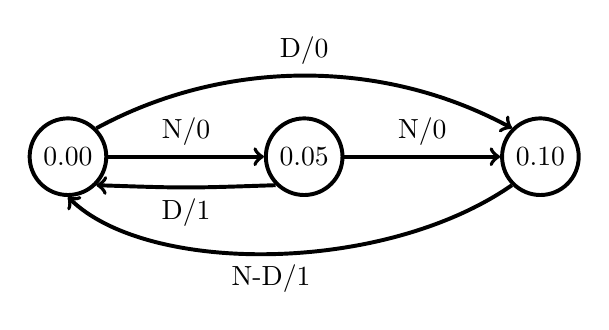
\begin{tikzpicture} [scale=1.00]
  \usepgflibrary{shapes.multipart} % for the multipart nodes
  % make all path lines (the node shapes) a little thicker
  \tikzstyle{every path}=[line width=0.50mm]  
  
  % Draw the lines
  \node [circle,draw] (00) at (2.00, 4) {$ 0.00 $};
  \node [circle,draw] (05) at (5.00, 4) {$ 0.05 $};
  \node [circle,draw] (10) at (8.00, 4) {$ 0.10 $};
  %  \node [circle,draw] (15) at (9.50, 4) {$ 0.15 $};
  
  % ``N'' Arrows
  \draw[->] (00.east) .. controls (3.50,4)  .. node[above] {N/$0$} (05.west);
  \draw[->] (05.east) .. controls (6.50,4)  .. node[above] {N/$0$} (10.west);
  
  % ``D'' Arrows
  \draw[->] (00.north east) .. controls (4.00,5.25) and (6.00,5.25)  .. node[above] {D/$0$} (10.north west);
  \draw[->] (05.south west) .. controls (3.50,3.60)  .. node[below] {D/$1$} (00.south east);
  
  % ``Vend'' Arrow
  \draw[->] (10.south west) .. controls (6.00,2.50) and (3.00,2.50)  .. node[below] {N-D/$1$} (00.south);  
  ;
  \end{tikzpicture}
\end{figure}

In Figure \ref{SIM:fig:mealy_vending_machine_fsm} the states are identified by the amount of money that has been deposited, so the first state on the left ($ 0.00 $) is when no money has been deposited. Following the path directly to the right of the first state, if five cents (indicated by ``N'' for a nickel) is deposited, then the output is zero (no candy is dispensed) and the state is changed to $ 0.05 $. If another five cents is deposited, the output remains zero and the state changes to $ 0.10 $. At that point, if either five or ten cents (``N'' or ``D'') is deposited, then the output changes to $ 1 $ (candy is dispensed) and the state resets to $ 0.00 $. By following the transition arrows various combinations of inputs and their resulting output can be traced.

Because the Mealy \ac{FSM} reacts immediately to any input it requires one less state than the Moore machine (compare Figures \ref{SIM:fig:moore_vending_machine_fsm} and \ref{SIM:fig:mealy_vending_machine_fsm}). However, since Moore machines only change states on a clock pulse they tend to be more predictable (and safer) when integrated into other modules. Finally, Mealy machines tend to react faster than Moore machines since they do not need to wait for a clock pulse and, generally, are implemented with fewer gates. In the end, whether to design with a Mealy or a Moore machine is left to the designer's discretion and, practically speaking, most designers tend to favor one type of \ac{FSM} over the other. The simulations in this book use Moore machines because they tend to be easier to understand and more stable in operation.

\subsection{Finite State Machine Tables}
\label{SIM:subsec:finite_state_machine_tables}

Many designers enjoy using Moore and Mealy \ac{FSM} diagrams as presented in Figures \ref{SIM:fig:moore_vending_machine_fsm} and \ref{SIM:fig:mealy_vending_machine_fsm}; however, others prefer to design with a finite state machine table that lists all states, inputs, and outputs. As an example, imagine a pedestrian crosswalk in the middle of a downtown block. The crosswalk has a traffic signal to stop traffic and a \emph{Cross / Don't Cross} light for pedestrians. It also has a button that pedestrians can press to make the light change so it is safe to cross.

This system has several states which can be represented in a \emph{State Table}. The traffic signal can be Red, Yellow, or Green and the pedestrian signal can be Walk or Don't Walk. Each of these signals can be either zero (for \emph{Off}) or one (for \emph{On}). Also, there are two triggers for the circuit; a push button (the \emph{Cross} button that a pedestrian presses) and a timer (so the walk light will eventually change to don't walk). If the button is assumed to be one when it is pressed and zero when not pressed, and the timer is assumed to be one when a certain time interval has expired but zero otherwise, then State Table \ref{SIM:tab:crosswalk_state_table} can be created.

\begin{table}[H]
  \sffamily
  \newcommand{\head}[1]{\textcolor{white}{\textbf{#1}}}    
  \begin{center}
    \rowcolors{2}{gray!10}{white} % Color every other line a light gray
    \begin{tabular}{ccccccccccccc} 
      \rowcolor{black!75}
      & \multicolumn{5}{c}{\head{Current State}} & \multicolumn{2}{c}{\head{Trigger}} & \multicolumn{5}{c}{\head{Next State}} \\
      & R & Y & G & W & D & Btn & Tmr & R & Y & G & W & D \\
      \hline
      1 & 0 & 0 & 1 & 0 & 1 & 0 & 0 & 0 & 0 & 1 & 0 & 1 \\
      2 & 0 & 0 & 1 & 0 & 1 & 1 & 0 & 0 & 1 & 0 & 0 & 1 \\
      3 & 0 & 1 & 0 & 0 & 1 & X & 0 & 1 & 0 & 0 & 1 & 0 \\
      4 & 1 & 0 & 0 & 1 & 0 & X & 1 & 0 & 0 & 1 & 0 & 1
    \end{tabular}
  \end{center}
  \caption{Crosswalk State Table}
  \label{SIM:tab:crosswalk_state_table}
\end{table}

The various states are $ R $ (for \emph{Red}), $ Y $ (for \emph{Yellow}), and $ G $ (for \emph{Green}) traffic lights, and $ W $ (for \emph{Walk}) and $ D $ (for \emph{Don't Walk}) pedestrian lights. The \emph{Btn} (for \emph{Cross Button}) and \emph{Tmr} (for \emph{Timer}) triggers can, potentially, change the state of the system. 

Row One on this table shows that the traffic light is Green and the pedestrian light is Don't Walk. If the button is not pressed (it is zero) and the timer is not active (it is zero), then the next state is still a Green traffic light and Don't Walk pedestrian light; in other words, the system is quiescent. In Row Two, the button was pressed (\emph{Btn} is one); notice that the traffic light changes state to Yellow, but the pedestrian light is still Don't Walk. In Row Three, the current state is a Yellow traffic light with Don't Walk pedestrian light (in other words, the \emph{Next State} from Row Two), the $ X $ for the button means it does not matter if it is pressed or not, and the next state is a Red traffic light and Walk pedestrian light. In Row Four, the timer expires (it changes to one at the end of the timing cycle), and the traffic light changes back to Green while the pedestrian light changes to Don't Walk. 

While Table \ref{SIM:tab:crosswalk_state_table} represents a simplified traffic light system, it could be extended to cover all possible states. Since Red, Yellow, and Green can never all be one at one time, nor could Walk and Don't Walk, the designer must specifically define all of the states rather than use a simple binary count from $ 00000 $ to $ 11111 $. Also, the designer must be certain that some combinations never happen, like a Green traffic light and a Walk pedestrian light at the same time, so those must be carefully avoided. 

State tables can be used with either Mealy or Moore machines and a designer could create a circuit that would meet all of the requirements from the state table and then realize that circuit to actually build a traffic light system. 

%***************************************************************************
% Section: Elevator
%***************************************************************************
\section{Elevator}
\label{SIM:sec:elevator}

As a simple example of a \ac{FSM}, imagine an elevator control circuit. For simplicity, this elevator is in a five story building and buttons like ``door open'' will be ignored. There are two ways the elevator can be called to a given floor: someone could push the floor button on the elevator to ride to that floor or someone could push the call button beside the elevator door on a floor.

 Figure \ref{SIM:fig:elevator} is the Moore \ac{FSM} for this circuit:

\begin{figure}[H]
  \caption{Elevator}
  \label{SIM:fig:elevator}
  \myfloatalign
  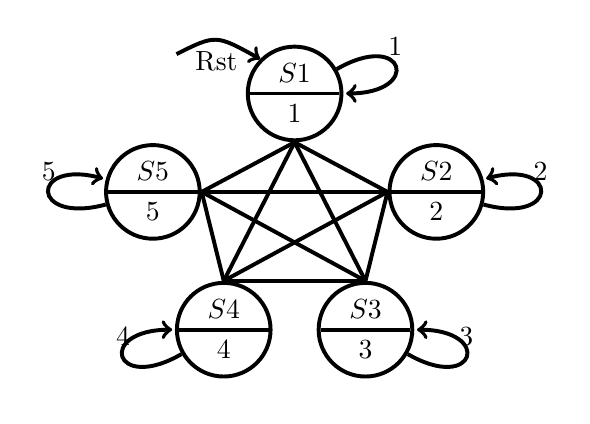
\begin{tikzpicture} [scale=1.00]
  \usepgflibrary{shapes.multipart} % for the multipart nodes
  % make all path lines (the node shapes) a little thicker
  \tikzstyle{every path}=[line width=0.50mm]  
  
  % Draw the lines
  \node [circle split,draw] (S1) at (4.00, 5.00) {$ S1 $ \nodepart{lower} $ 1 $};
  \node [circle split,draw] (S2) at (5.80, 3.75) {$ S2 $ \nodepart{lower} $ 2 $};
  \node [circle split,draw] (S3) at (4.90, 2.00) {$ S3 $ \nodepart{lower} $ 3 $};
  \node [circle split,draw] (S4) at (3.10, 2.00) {$ S4 $ \nodepart{lower} $ 4 $};
  \node [circle split,draw] (S5) at (2.20, 3.75) {$ S5 $ \nodepart{lower} $ 5 $};
  
  % edge connectors
  \draw (S1.south) -- (S2.west);
  \draw (S2.west)  -- (S3.north);
  \draw (S3.north) -- (S4.north);
  \draw (S4.north) -- (S5.east);
  \draw (S5.east)  -- (S1.south);
  % cross connectors
  \draw (S1.south) -- (S3.north);
  \draw (S1.south) -- (S4.north);
  \draw (S2.west)  -- (S5.east);
  \draw (S2.west)  -- (S4.north);
  \draw (S3.north) -- (S5.east);

  % Loops
  \draw (S1) edge [in=0,out=30,loop] node[above] {1} ();
  \draw (S2) edge [in=15,out=345,loop] node[above] {2} ();
  \draw (S3) edge [in=0,out=330,loop] node[above] {3} ();
  \draw (S4) edge [in=180,out=210,loop] node[above] {4} ();
  \draw (S5) edge [in=165,out=195,loop] node[above] {5} ();
  
  % Reset input
  \draw[->] (2.50,5.50) .. controls (3.00,5.75) .. node[below] {Rst}  (S1.north west);
    

  \end{tikzpicture}
\end{figure}

In Figure \ref{SIM:fig:elevator} the various floors are represented by the five states (S1-S5). While the elevator is at a floor then the output from the circuit is the floor number. The elevator is quiescent while in any one state and if a user pushes the button for that same floor then nothing will happen, which is illustrated by the loops starting and coming back to the same state. The star pattern in the middle of the \ac{FSM} illustrates that the elevator can move directly from one state to any other state. Finally, a Reset signal will automatically move the elevator to state S1.


%***************************************************************************
% Section: CPU
%***************************************************************************
\section{Central Processing Unit}
\label{SIM:sec:cpu}

\subsection{Introduction}
\label{SIM:subsec:intro_to_cpu}

The \acf{CPU} is the core of any computer, tablet, phone, or other computer-like device. While many definitions of \ac{CPU} have been offered, many quite poetic (like the ``heart'' or ``brain'' of a computer); probably the best definition is that the \ac{CPU} is the intersection of software and hardware. The \ac{CPU} contains circuitry that converts the ones and zeros that are stored in memory (a ``program'') into controlling signals for hardware devices. The \ac{CPU} retrieves and analyzes bytes that are contained in a program, turns on or off multiplexers and control buffers so data are moved to or from various devices in the computer, and permits humans to use a computer for intellectual work. In its simplest form, a \ac{CPU} does nothing more than fetch a list of instructions from memory and then execute those instructions one at a time. This chapter explores \acp{CPU} from a theoretical perspective.

\subsubsection{Concepts}

A \ac{CPU} processes a string of ones and zeros and uses the information in that binary code to enable/disable circuits or hardware devices in a computer system. For example, a \ac{CPU} may execute a binary code and create electronic signals that first place data on the computer's data bus and then spins up the hard drive to store that data. As another example, perhaps the \ac{CPU} detects a key press on a keyboard, transfers that key's code to memory and also sends a code to the monitor where specific pixels are activated to display the letter pressed.

Figure \ref{sim:fig:simple_data_flow_control_circuit} illustrates a very simple circuit used to control the flow of data on a data bus.

\begin{figure}[H]
  \caption{Simple Data Flow Control Circuit}
  \label{sim:fig:simple_data_flow_control_circuit}  
  \myfloatalign
  \begin{tikzpicture} [circuit logic US, scale=1.00]
  % make all path lines (the node shapes) a little thicker
  \tikzstyle{every path}=[line width=0.50mm]
  
  % Keyboard
  \node[minimum width=2.0cm,draw] (g01) at (5.00,4.00) {Keyboard};
  \node[] (kbd) at (4.15,4.00) {};

  % Monitor
  \node[minimum width=2.0cm,draw] (g02) at (5.00,3.00) {Monitor};
  \node[] (mon) at (4.15,3.00) {};
  
  % Memory
  \node[minimum size=2.0cm,draw] (g03) at (5.00,1.00) {Memory};
  \node[] (min) at (4.15,1.50) {};
  \node[] (mot) at (4.15,0.50) {};
  
  % Buffers
  \node[buffer,inputs={n},scale=0.5,rotate=180] (buf_01) at (3.50,4.0) {};
  \node[buffer,inputs={n},scale=0.5]            (buf_02) at (3.50,3.0) {};
  \node[buffer,inputs={n},scale=0.5]            (buf_03) at (3.50,1.5) {};
  \node[buffer,inputs={n},scale=0.5,rotate=180] (buf_04) at (3.50,0.5) {};

  % Demux
  \node[trapezium,rotate=90,minimum size=1.0cm,draw] (g04) at (1.00,1.00) {};
  \node[label={[label distance=-0.55cm]0:$1$}] (1in) at (0.0,1.00) {};
  \node[label={[font=\scriptsize,label distance=-0.35cm]0:Din}] (n1) at (0.65,1.00) {};
  \node[label={[font=\scriptsize,label distance=-0.35cm]180:A}] (oA) at (1.35,1.35) {};
  \node[label={[font=\scriptsize,label distance=-0.35cm]180:B}] (oB) at (1.35,0.65) {};
  \node[label={[font=\scriptsize,label distance=-0.50cm]270:S}] (S) at (0.80,0.50) {};
  
  % Labels
  \node[circle,pin=135:Data] at (2.75,4) {};
  \node[circle,pin=135:A] at (1.85,3.55) {};
  \node[circle,pin=225:B] at (2.25,0.00) {};
  
  % Draw the lines
  \draw
  
  (1in) -- (n1)
  (0.8,0.0) -- (S)
  
  % Data Bus
  (2.75,0.5) -- (2.75,4)
  (2.75,4.0) -- (buf_01.out)
  (2.75,3.0) -- (buf_02.in)
  (2.75,1.5) -- (buf_03.in)
  (2.75,0.5) -- (buf_04.out)
  
  % Connect buffers to devices
  (kbd) -- (buf_01.in)
  (mon) -- (buf_02.out)
  (min) -- (buf_03.out)
  (mot) -- (buf_04.in)

  % Dmux A to Kbd+mem
  (oA) -- (1.85,1.35)
  (1.85,1.35) -- (1.85,3.55) -- (3.50,3.55)
  (1.85,1.35) -- (1.85,0.95) -- (3.50,0.95)
  (3.50,3.85) -- (3.50,3.55) % Ctrl out of Buf 1
  (3.50,1.30) -- (3.50,0.95) % Ctrl out of Buf 3

  % Dmux B to Mon+mem
  (oB) -- (2.25,0.65)
  (2.25,0.65) -- (2.25,2.45) -- (3.50,2.45)
  (2.25,0.65) -- (2.25,0.00) -- (3.50,0.00)
  (3.50,2.80) -- (3.50,2.45) % Ctrl out of Buf 2
  (3.50,0.30) -- (3.50,0.00) % Ctrl out of Buf 4

  ;
  \end{tikzpicture}
\end{figure}

In Figure \ref{sim:fig:simple_data_flow_control_circuit}, the demultiplexer at the bottom left corner of the circuit controls four control buffers that, in turn, control access to the data bus. When output $ A $ is active then input from the Keyboard is stored in Memory; but when output $ B $ is active then output from memory is sent to the monitor. By setting the select bit in the demultiplexer the circuit's function can be changed from reading the keyboard to writing to the monitor using a single data bus.

In a true \ac{CPU}, of course, there are many more peripheral devices, along with an \ac{ALU}, registers, and other internal resources to control. Figure \ref{sim:fig:simplified_cpu_block_diagram} is a block diagram for a simplified \ac{CPU}.

\begin{figure}[H]
  \caption{Simplified CPU Block Diagram}
  \label{sim:fig:simplified_cpu_block_diagram}
  \myfloatalign
  \begin{tikzpicture} [circuit logic US, scale=1.00]
  % make all path lines (the node shapes) a little thicker
  \tikzstyle{every path}=[line width=0.50mm]
  
  % Blocks
  \node[minimum width=3.5cm,draw] (blk01) at (4.00,6.00) {Control};
  \node[minimum width=3.5cm,draw] (blk02) at (4.00,5.00) {ALU};
  \node[minimum width=3.5cm,draw] (blk03) at (4.00,4.00) {General Regs};
  \node[minimum width=3.5cm,draw] (blk04) at (4.00,3.00) {Program Counter};
  \node[minimum width=3.5cm,draw] (blk05) at (4.00,2.00) {Address Reg};
  \node[minimum width=3.5cm,draw] (blk06) at (4.00,0.75) {RAM};
  \node[minimum width=3.5cm,draw] (blk07) at (9.00,3.50) {Peripherals};

  % The block nodes 
  \node[] (blk01e) at (2.42,6.00) {};
  \node[] (blk02e) at (2.42,5.00) {};
  \node[] (blk03e) at (2.42,4.00) {};
  \node[] (blk04e) at (2.42,3.00) {};
  \node[] (blk05e) at (2.42,2.00) {};
  \node[] (blk06e) at (2.42,0.75) {};

  \node[] (blk01w) at (5.58,6.00) {};
  \node[] (blk02w) at (5.58,5.00) {};
  \node[] (blk03w) at (5.58,4.00) {};
  \node[] (blk04w) at (5.58,3.00) {};
  \node[] (blk05w) at (5.58,2.00) {};
  \node[] (blk06w) at (5.58,0.75) {};
  
  \node[] (blk05s) at (4.00,1.80) {};
  \node[] (blk06n) at (4.00,0.85) {};
    
  % Labels
  \node[circle,pin=135:Control] at (1.5,4) {};
  \node[circle,pin=45:Data]     at (6.5,4) {};
  \node[circle,pin=180:Address] at (4.00,1.35) {};
  
  % Draw the lines
  \draw
  (6.5,0.75) -- (6.5,6.0) % Data Bus Line
  (1.5,0.75) -- (1.5,6.0) % Control Bus Line
  ;

  % Arrows to Data Bus
  \draw[<->](blk01w) -- (6.5,6.0);
  \draw[<->](blk02w) -- (6.5,5.0);
  \draw[<->](blk03w) -- (6.5,4.0);
  \draw[<->](blk04w) -- (6.5,3.0);
  \draw[<-] (blk05w) -- (6.5,2.0);
  \draw[<->](blk06w) -- (6.5,0.75);

  % Arrows to Control Bus
  \draw[->](blk01e)   -- (1.5,6.0);
  \draw[->](1.5,5.0)  -- (blk02e);
  \draw[->](1.5,4.0)  -- (blk03e);
  \draw[->](1.5,3.0)  -- (blk04e);
  \draw[->](1.5,2.0)  -- (blk05e);
  \draw[->](1.5,0.75) -- (blk06e);

  \draw[<->](6.5,3.5) -- (7.25,3.5); % Arrow to peripherals block


  \draw[->](blk05s) -- (blk06n); % Arrow between addr and RAM blocks
  ;
  \end{tikzpicture}
\end{figure}

The \ac{CPU} in Figure \ref{sim:fig:simplified_cpu_block_diagram} has three bus lines: 

\begin{itemize}
  \item \textsc{Control}. This bus contains all of the signals needed to activate control buffers, multiplexers, and demultiplexers in order to move data.
  \item \textsc{Data}. This contains the data being manipulated by the \ac{CPU}.
  \item \textsc{Address}. This is the address for the next instruction to fetch from \ac{RAM}.
\end{itemize}

There are several blocks in the \ac{CPU} in Figure \ref{sim:fig:simplified_cpu_block_diagram}:

\begin{itemize}
  \item \textsc{Control}. This block contains the circuitry necessary to decode an instruction that was fetched from \ac{RAM} and then activate the various devices needed to control the flow of data within the \ac{CPU}.
  \item \textsc{\ac{ALU}}. This is an \acl{ALU} designed for the application that is using this \ac{CPU}.
  \item \textsc{General Registers}. Most \acp{CPU} include a number of general registers that temporarily hold binary numbers or instructions.
  \item \textsc{Program Counter}. This is a register that contains the address of the next instruction to fetch from \ac{RAM}.
  \item \textsc{Address Register}. This contains the address for the current \ac{RAM} operation.
  \item \textsc{\ac{RAM}}. While most computers and other devices have a large amount of \ac{RAM} outside the \ac{CPU}, many \acp{CPU} are constructed with a small amount of internal \ac{RAM} for increased operational efficiency. This type of high-speed \ac{RAM} is usually called cache (pronounced ``cash'').
\end{itemize}

In operation, the \ac{CPU} moves the value of the Program Counter to the Address Register and then fetches the instruction contained at that \ac{RAM} address. That instruction is then sent to the Control circuit where it is decoded. The Control circuit activates the appropriate control devices to execute the instruction. This process is repeated millions of times every second while the \ac{CPU} executes a program.

\subsubsection{History}

\acp{CPU} from the early days of computing (circa $ 1950 $) were custom made for the computer on which they were found. Computers in those early days were rather rare and there was no need for a general-purpose \ac{CPU} that could function on multiple platforms. By the $ 1960 $s \emph{IBM} designed a family of computers based on the design of the \emph{System/$ 360 $}, or \emph{S/$ 360 $}. The goal was to have a number of computers use the same \ac{CPU} so programs written for one computer could be executed on another in the same family. By doing this, \emph{IBM} hoped to increase their customer loyalty.

\acp{CPU} today can be divided into two broad groups: \ac{CISC} (pronounced like ``sisk'') and \ac{RISC}. Early computers, like the IBM S/$ 360 $ had a large, and constantly growing, set of instructions, and these types of \acp{CPU} were referred to as \ac{CISC}. However, building the circuits needed to execute all of those instructions became ever more challenging until, in the late $ 1980 $s, computer scientists began to design \ac{RISC} \acp{CPU} with fewer instructions. Because there were fewer \ac{CPU} instructions circuits could be smaller and faster, but the trade off was that occasionally a desired instruction had to be simulated by combining two or more other instructions, and that creates longer, more complex computer programs. Nearly all computers, cell phones, tablets, and other computing devices in use today use a \ac{RISC} architecture.

More recent developments in \acp{CPU} include ``pipelining'' where the \ac{CPU} can execute two or more instructions simultaneously by overlapping them, that is, fetching and starting an instruction while concurrently finishing the previous instruction. Another innovation changed compilers such that they can create efficient \ac{VLIW} codes that combine several instructions into a single step. Multi-threading \acp{CPU} permit multiple programs to execute simultaneously and multi-core \acp{CPU} use multiple \ac{CPU} cores on the same substrate so programs can execute in parallel. 

\acp{CPU}, indeed, all hardware devices, are normally designed using an \ac{HDL} like Verilog to speed development and ensure high quality by using peer review before an \ac{IC} is manufactured. It is possible to find Open Source Verilog scripts for many devices, including \ac{CPU} cores\footnote{\url{http://www.opencores.org}}, so designers can begin with mature, working code and then ``tweak'' it as necessary to match their particular project.

\subsubsection{CPU Design Principles}

\ac{CPU} design commonly follows these steps:

\paragraph{Analysis of Intended Use} Designing a \ac{CPU} starts with an analysis of its intended use since that will determine the type of \ac{CPU} that must be built. A simple four-bit \ac{CPU} --- that is, all instructions are only four-bits wide --- is more than adequate for a simple device like a microwave oven, but for a cell phone or other more complex device, a 16-bit, or larger, \ac{CPU} is needed. 

\paragraph{The Instruction Set} After the purpose of the \ac{CPU} is defined then an instruction set is created. \ac{CPU} instructions control the physical flow of bits through the \ac{CPU} and various components of a computer. While an instruction set looks something like a programming language, it is important to keep in mind that an instruction set is very different from the more familiar higher-level programming languages like \emph{Java} and \emph{C++}.

\ac{CPU} instructions are 16-bit (or larger) words that are conceptually divided into two sections: the operational code (\emph{opcode}) and data. There are several classes of instructions, but three are the most common: 

\begin{itemize}
  \item \textsc{R (Register)}. These instructions involve some sort of register activity. The quintessential R-Type instruction is \lstinline[columns=fixed]|ADD|, where the contents of two registers are added together and the sum is placed in another register.
  \item \textsc{I (Immediate)}. These instructions include data as part of the instruction word and something happens immediately with that data. As an example, the \lstinline[columns=fixed]|LDI| instruction immediately loads a number contained in the instruction word into a specified register.
  \item \textsc{J (Jump)}. These instructions cause the program flow to jump to a different location. In older procedural programming languages (like \emph{C} and \emph{Basic}) these were often called \lstinline[columns=fixed]|GOTO| statements.
\end{itemize}

\paragraph{Assembly Language} A computer program is nothing more than a series of ones and zeros organized into words the bit-width of the instruction set,  commonly $ 32 $-bit or $ 64 $-bit. Each word is a single instruction and a series of instructions forms a program in \emph{machine code} that looks something like this:

\begin{align}
  \label{SIM:eq:sample_machine_code}
  0000 0000 0000 0000\\
  \nonumber
  1001 0001 0000 1010\\
  \nonumber
  1001 0010 0000 1001\\
  \nonumber
  0111 0011 0001 1000\\
  \nonumber
  0110 0000 0010 0011
\end{align}

A \ac{CPU} fetches and executes one $ 16 $-bit word of the machine code at a time. If a programmer could write machine code directly then the \ac{CPU} could execute it without needing to compile it first. Of course, as it is easy to imagine, no one actually writes machine code due to its complexity. 

The next level higher than machine code is called \emph{Assembly}, which uses easy-to-remember abbreviations (called ``mnemonics'') to represent the available  instructions. Following is the assembly language program for the machine code listed above:

\begin{verbatim}
  Label Mnemonic Operands    Comment
  START NOP      0 0 0       No Operation
        LDI      1 0 a       R1  <- 0ah
        LDI      2 0 9       R2  <- 09h
        SHL      3 1 4       R3  <- R1 << 8
        XOR      0 2 3       Acc <- R2 XOR R3
\end{verbatim}

Each line of assembly has four parts. First is an optional \emph{Label} that can be used to indicate various sections of the program and facilitates ``jumps'' around the program; second is the mnemonic for the code being executed; third are one or more operands; and fourth is an optional comment field.

\marginpar{Machine code is \ac{CPU} specific so code written for one type of computer could not be used on any other type of computer.} 

Once the program has been written in Assembly, it must be ``assembled'' into machine code before it can be executed. An assembler is a fairly simply program that does little more than convert a file containing assembly code into instructions that can be executed by the \ac{CPU}. The assembly program presented above would be assembled into Machine Code \ref{SIM:eq:sample_machine_code}.

\paragraph{Programming Languages}

Many high level programming languages have been developed, for example \emph{Java} and \emph{C++}. These languages tend to be easy to learn and can enable a programmer to quickly create very complex programs without digging into the complexity of machine code.

Programs written in any of these high-level languages must be either interpreted or compiled before they can be executed. Interpreters are only available for ``scripting'' languages like \emph{PERL} and \emph{Python} and they execute the source code one line at a time. In general, interpreters cannot optimize the code so they are not efficient; but they enable a programmer to quickly ``try out'' some bit of code without having to compile it. A compiler, on the other hand, converts the entire program to machine code (normally referred to as ``object'' code by a compiler) and then creates an executable file. A compiler also optimizes the code so it executes as efficiently as possible.

In the end, there are dozens of different programming languages, but they all eventually reduce programming instructions to a series of ones and zeros which the \ac{CPU} can execute.

\subsubsection{State Machine}

Because a \ac{CPU} is little more than a complex \ac{FSM}, the next step in the design process is to define the various states and the operations that take place within each state. In general, an operating \ac{CPU} cycles endlessly through three primary states:

\begin{itemize}
  \item \textsc{Fetch} an instruction from memory. Instructions take the form of 16-bit numbers similar in appearance to $ 1001 0001 0000 1010 $.
  \item \textsc{Decode} the instruction. The instruction fetched from memory must be decoded into something like ``Add the contents of Register $ 2 $ to Register $ 3 $ and save the results in Register 1.''
  \item \textsc{Execute} the instruction.
\end{itemize}

In general, the way that a \ac{CPU} functions is to fetch a single instruction from \ac{RAM} and then decode and execute that instruction. As an example, consider the Assembly example introduced above:

\begin{Verbatim}[commandchars=~\[\], samepage=true, fontfamily=courier]
Label Mnemonic Operands    Comment
START NOP      0 0 0       No Operation
      LDI      1 0 a       R1  <- 0ah
      LDI      2 0 9       R2  <- 09h
      SHL      3 1 4       R3  <- R1 << 8
      XOR      0 2 3       Acc <- R2 XOR R3
\end{Verbatim}

Each line is an instruction and the \ac{CPU} would fetch and execute each instruction from \ac{RAM} in order. The purpose of this short code snip is to load a $ 16 $-bit register with a number when only $ 8 $ bits are available in the opcode. The eight high order bits are loaded into Register one and the eight low order bits are loaded into Register two. The high order bits are shifted to the left eight places and then the two registers are \lstinline[columns=fixed]|XOR|'d together:

\begin{enumerate}
  \item \lstinline[columns=fixed]|NOP|: This is a ``no operation'' instruction so the \ac{CPU} does nothing.
  \item \lstinline[columns=fixed]|LDI|: The number $ 0A_{16} $ is loaded into register one. This is the value of the high-order bits desired in the $ 16 $-bit number.
  \item \lstinline[columns=fixed]|LDI|: The number $ 09_{16} $ is loaded into register two.  This is the value of the low-order bits desired in the $ 16 $-bit number.
  \item \lstinline[columns=fixed]|SHL|: Register three is loaded with the value of register one shifted left eight places.
  \item \lstinline[columns=fixed]|XOR|: The Accumulator is loaded with the value of register two \lstinline[columns=fixed]|XOR|'d with 4egister three. This leaves the accumulator with a \lstinline[columns=fixed]|16|-bit number, $ 0A09_{16} $ that was loaded eight bits at a time.
\end{enumerate}

\subsection{CPU States}
\label{SIM:subsec:cpu_states}

The first task that a \ac{CPU} must accomplish is to fetch and decode an instruction held in memory. Figure \ref{SIM:fig:cpu_state_diagram} is a simplified state diagram that shows the first two \ac{CPU} states as \emph{Fetch} and \emph{Decode}. After that, all of the different instructions would create their own state (for simplicity, only three instructions are shown in the Figure \ref{SIM:fig:cpu_state_diagram}).

\begin{figure}[H]
  \caption{CPU State Diagram}
  \label{SIM:fig:cpu_state_diagram}
  \myfloatalign
  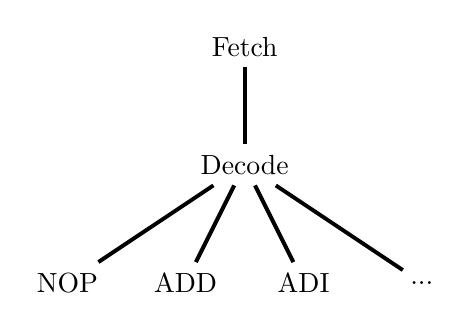
\begin{tikzpicture} [scale=1.00]
  \usepgflibrary{shapes.multipart}
  \usetikzlibrary{trees} 
  % make all path lines (the node shapes) a little thicker
  \tikzstyle{every path}=[line width=0.50mm]  
  
  \node(F0) {Fetch}
    child {node {Decode}
      child {node {NOP}}
      child {node {ADD}}
      child {node {ADI}}
      child {node {...}}
    };
  ;
  \end{tikzpicture}
\end{figure}

The \ac{CPU} designer would continue to design states for all instructions and end each state with a loop back to Fetch in order to get the next instruction out of \ac{RAM}.

Designing a \ac{CPU} is no insignificant task and is well beyond the scope of this book. However, one of the labs in the accompanying lab manual design a very simple processor that demonstrates how bits are moved around a circuit based upon control codes.